%% abtex2-modelo-slides.tex, v-1.0 gfabinhomat
%% Copyright 2012-2016 by abnTeX2 group at http://www.abntex.net.br/ 
%%
%% This work may be distributed and/or modified under the
%% conditions of the LaTeX Project Public License, either version 1.3
%% of this license or (at your option) any later version.
%% The latest version of this license is in
%%   http://www.latex-project.org/lppl.txt
%% and version 1.3 or later is part of all distributions of LaTeX
%% version 2005/12/01 or later.
%%
%% This work has the LPPL maintenance status `maintained'.
%% 
%% The Current Maintainer of this work is Fábio Rodrigues Silva, 
%% member of abnTeX2 team, led by Lauro César Araujo. 
%% Further information are available on 
%% http://www.abntex.net.br/
%%
%% This work consists of the files abntex2-modelo-slides.tex, 
%% abntex2-modelo-references.bib and abntex2-modelo-marca.pdf
%%
%% Modelo desenvolvido por Fábio Rodrigues Silva (gfabinhomat@gmail.com)
%% Mais informações podem ser obtidas no guia do usuário Beamer 
%% (http://linorg.usp.br/CTAN/macros/latex/contrib/beamer/doc/beameruserguide.pdf)
%% Informações rápidas podem ser acessadas em http://en.wikibooks.org/wiki/LaTeX/Presentations


% Apresentações em widescreen. Outros valores possíveis: 1610, 149, 54, 43 e 32.
% Por padrão, as apresentações são no formato 4:3 (sem o aspectratio).
\documentclass[aspectratio=1610]{beamer}	 	

\everymath{\displaystyle} %farc tamanho ideal
\usetheme{Pittsburgh}
\usecolortheme{default}
\usefonttheme[onlymath]{serif}			% para fontes matemáticas
% Enconte mais temas e cores em http://www.hartwork.org/beamer-theme-matrix/ 
% Veja também http://deic.uab.es/~iblanes/beamer_gallery/index.html

% Customizações de Cores: fg significa cor do texto e bg é cor do fundo
\setbeamercolor{normal text}{fg=black}
\setbeamercolor{alerted text}{fg=red}
\setbeamercolor{author}{fg=darkgray}
\setbeamercolor{institute}{fg=blue}
\setbeamercolor{date}{fg=green}
\setbeamercolor{frametitle}{fg=blue}
\setbeamercolor{framesubtitle}{fg=brown}
\setbeamercolor{block title}{bg=blue, fg=white}		%Cor do título
\setbeamercolor{block body}{bg=lightgray, fg=darkgray}	%Cor do texto (bg= fundo; fg=texto)

% ---
% PACOTES
% ---
\usepackage[alf]{abntex2cite}		% Citações padrão ABNT
\usepackage[brazil]{babel}		% Idioma do documento
\usepackage{color}			% Controle das cores
\usepackage[T1]{fontenc}		% Selecao de codigos de fonte.
\usepackage{graphicx}			% Inclusão de gráficos
\usepackage[utf8]{inputenc}		% Codificacao do documento (conversão automática dos acentos)
\usepackage{txfonts}			% Fontes virtuais
% ---

% --- Informações do documento ---
\title{Comparação entre Julia e outras linguagens de programação na eficiência de execução do método de Newton-Raphson para solução de sistema de equações não-lineares}
\author{{\scriptsize André Rodrigues Bezerra Madruga \\ 
		Bruno Matias de Sousa \\ 
		José Ricardo Bezerra de Araújo \\ 
		Levy Gabriel da Silva Galvão \\}}
\date{\today}
% ---

% ----------------- INÍCIO DO DOCUMENTO --------------------------------------
\begin{document}

% ----------------- NOVO SLIDE --------------------------------
\begin{frame}

\begin{minipage}{1\linewidth}
  \centering
    %
\includegraphics[width=1cm]{ufrn.jpg} \\
	\begin{footnotesize}
	 \textbf{Universidade Federal do Rio Grande do Norte} \\ 
	\textbf{Centro de Tecnologia} \\ 
	\textbf{Departamento de Engenharia da Computação e Automação} \\ 
	\textbf{DCA0304 -- Métodos Computacionais em Engenharia} \\
	 \end{footnotesize} 
\end{minipage}

\titlepage

\end{frame}

% ----------------- NOVO SLIDE --------------------------------
\begin{frame}{Sumário}
\tableofcontents
\end{frame}

% ----------------- NOVO SLIDE --------------------------------
\section{Introdução}

\begin{frame}{Introdução}

\begin{itemize}
 \item Vários problemas sem solução analítica; \pause
 
 \item Necessidade de métodos iterativos;\pause
 
 \item Computação numérica;\pause
 
 \item Várias linguagens de programação;\pause
 
 \item Julia: recente e eficiente.
\end{itemize}

\end{frame}

% ----------------- NOVO SLIDE --------------------------------
\section{Objetivos}

\begin{frame}{Objetivos}

\begin{itemize}
 \item Solução de sistemas de equações não-lineares pelo método de Newton-Raphson; \pause
 
 \item Utilizar \textit{Fortran 95}, \textit{Julia} e \textit{Python};\pause
 
 \item Comparar a eficiência de execução do algoritmo por cada linguagem;

\end{itemize}

\end{frame}

% ----------------- NOVO SLIDE --------------------------------

\begin{frame}{Sistemas de equações não-lineares}

\begin{block}{Sistema 1:}
 \begin{enumerate}
 \item $ x_2 + x_3 - e^{-x_1} = 0$
 \item $ x_1 + x_3 - e^{-x_3} = 0$
 \item $ x_1 + x_2 - e^{-x_3} = 0$
\end{enumerate}
\end{block}

\begin{block}{Sistema 2:}
 \begin{enumerate}
 \item $ \frac{1}{2}sen(x_1x_2) - \frac{x_2}{4\pi} - \frac{x_1}{2}  = 0$
 \item $ (1-\frac{1}{4\pi})(e^{2x_1}-e) - \frac{ex_2}{\pi} - 2ex_1 = 0$
\end{enumerate}
\end{block}


\end{frame}

% ----------------- NOVO SLIDE --------------------------------
\section{Implementação}
\begin{frame}
\frametitle{Fluxograma}


\begin{figure}
  \centering
  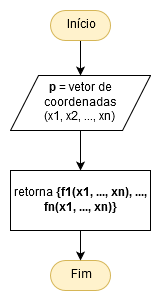
\includegraphics[scale=0.6]{Imagens/diag_func.png}
  \caption{Fluxograma da função f().}
\end{figure}


\end{frame}

% ----------------- NOVO SLIDE --------------------------------

\begin{frame}
\frametitle{Fluxograma}


\begin{figure}
  \centering
  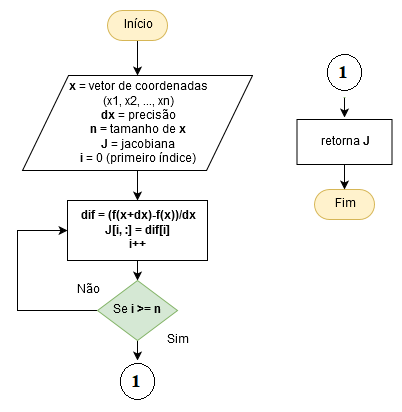
\includegraphics[scale=0.6]{Imagens/diag_jac1.png}
  \caption{Fluxograma da função jac().}
\end{figure}


\end{frame}

% ----------------- NOVO SLIDE --------------------------------

\begin{frame}
\frametitle{Fluxograma}


\begin{figure}
  \centering
  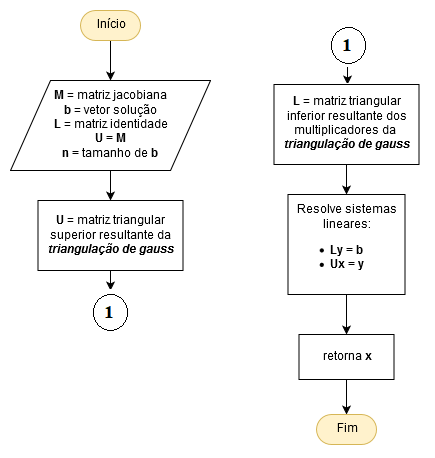
\includegraphics[scale=0.6]{Imagens/diag_LU1.png}
  \caption{Fluxograma da função LU().}
\end{figure}


\end{frame}


% ----------------- NOVO SLIDE --------------------------------

\begin{frame}
\frametitle{Fluxograma}


\begin{figure}
  \centering
  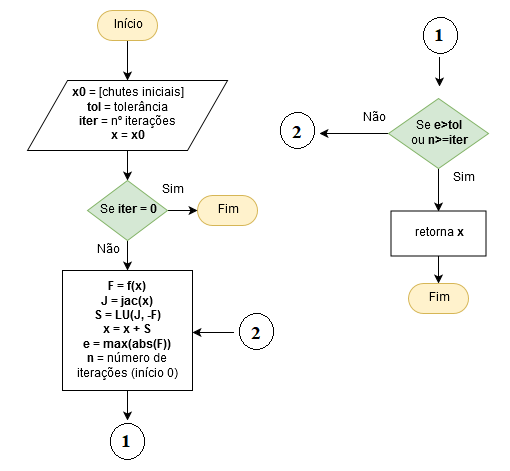
\includegraphics[scale=0.6]{Imagens/diag_new1.png}
  \caption{Fluxograma da função newrap().}
\end{figure}


\end{frame}

% ----------------- NOVO SLIDE --------------------------------

\begin{frame}
\frametitle{Fluxograma}


\begin{figure}
  \centering
  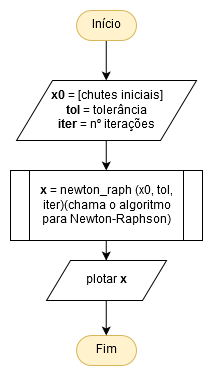
\includegraphics[scale=0.55]{Imagens/diag_main.png}
  \caption{Fluxograma da main.}
\end{figure}


\end{frame}


% ----------------- NOVO SLIDE --------------------------------
\begin{frame}

\begin{figure}
  \centering
  
\includegraphics[width=2cm]{ufrn.jpg}
  \caption{Marca abnTeX2. Fonte: \url{http://www.abntex.net.br/}}
\end{figure}

\end{frame}

% ----------------- NOVO SLIDE --------------------------------
\section{Resultados}


\begin{frame}
\frametitle{Tempo de execução}


\begin{figure}
  \centering
  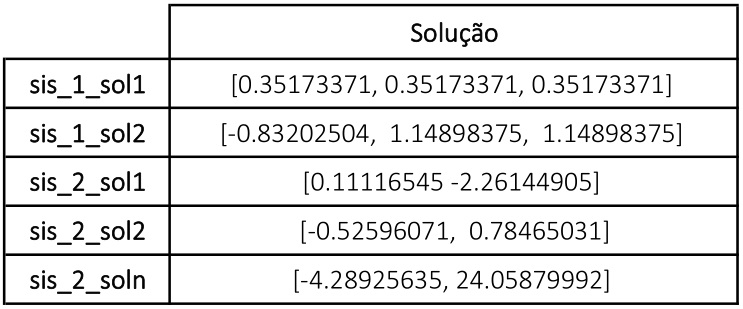
\includegraphics[scale=0.55]{Imagens/sol.jpg}
  \caption{Tabela de soluções para cada sistema.}
\end{figure}


\end{frame}


% ----------------- NOVO SLIDE --------------------------------

\begin{frame}
\frametitle{Tempo de execução}


\begin{figure}
  \centering
  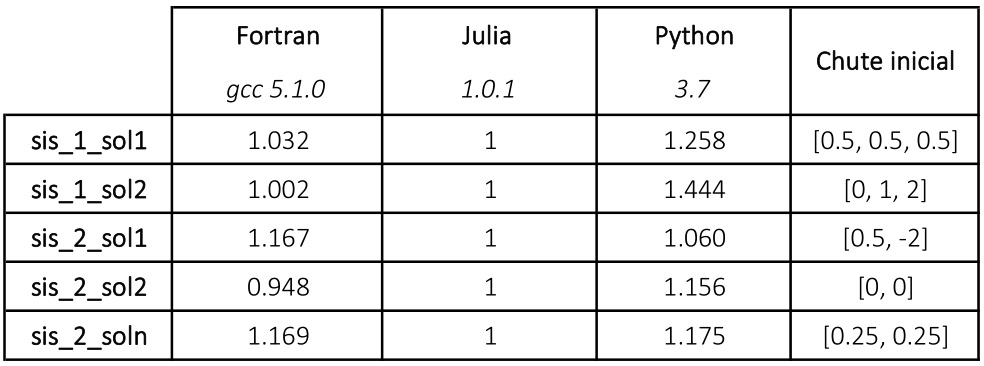
\includegraphics[scale=0.55]{Imagens/exe_rel.jpg}
  \caption{Tabela de comparação de tempo de execução relativo, tendo o tempo de Julia como 1.}
\end{figure}


\end{frame}

% ----------------- NOVO SLIDE --------------------------------

\begin{frame}
\frametitle{Tempo de execução}


\begin{figure}
  \centering
  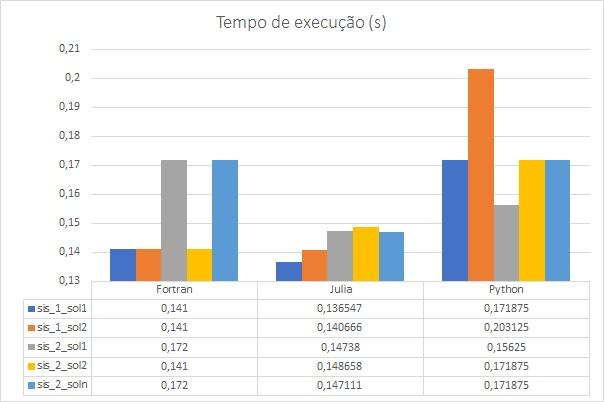
\includegraphics[scale=0.55]{Imagens/graf.jpg}
  \caption{Gráfico e tabela de comparação do tempo de execução absoluto.}
\end{figure}


\end{frame}


% ----------------- NOVO SLIDE --------------------------------

\begin{frame}
\frametitle{Tempo de execução}


\begin{figure}
  \centering
  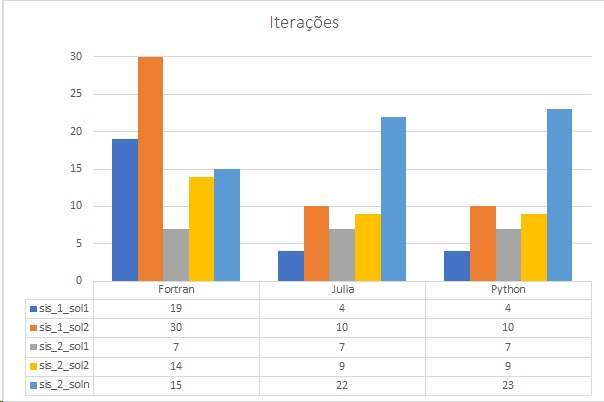
\includegraphics[scale=0.55]{Imagens/iter.jpg}
  \caption{Tabela de comparação de iterações.}
\end{figure}


\end{frame}


% ----------------- NOVO SLIDE --------------------------------
\section{Conclusões}

\begin{frame}{Conclusões}

\begin{itemize}
 \item Vários problemas sem solução analítica;
 
 \item Necessidade de métodos iterativos;
 
 \item Computação numérica;
 
 \item Várias linguagens de programação;
 
 \item Julia: recente e eficiente.
\end{itemize}

\end{frame}

% ----------------- FIM DO DOCUMENTO -----------------------------------------
\end{document}
